% build using lualatex-dev in TeXLive 2024 or later

\DocumentMetadata{
  uncompress,
  lang        = en,
  pdfversion  = 2.0,
  pdfstandard = ua-2,
  pdfstandard = a-4f, %or a-4
  testphase   = latest
}

\documentclass{article}

\usepackage[osf]{libertinus}
\usepackage{graphicx}
\usepackage{unicode-math}


\begin{document}

\title{Demo document}
\maketitle


\section{Start}
Body text.


% While most tagging is done automatically by adding the \DocumentMetadata
% command, there remain a few things the author has to add manually. At first
% every graphic must be marked either as artifact or get an alternative text
% describing its meaning in the context of the document. This can be done with
% additional keys that have been added to the \includegraphics command:

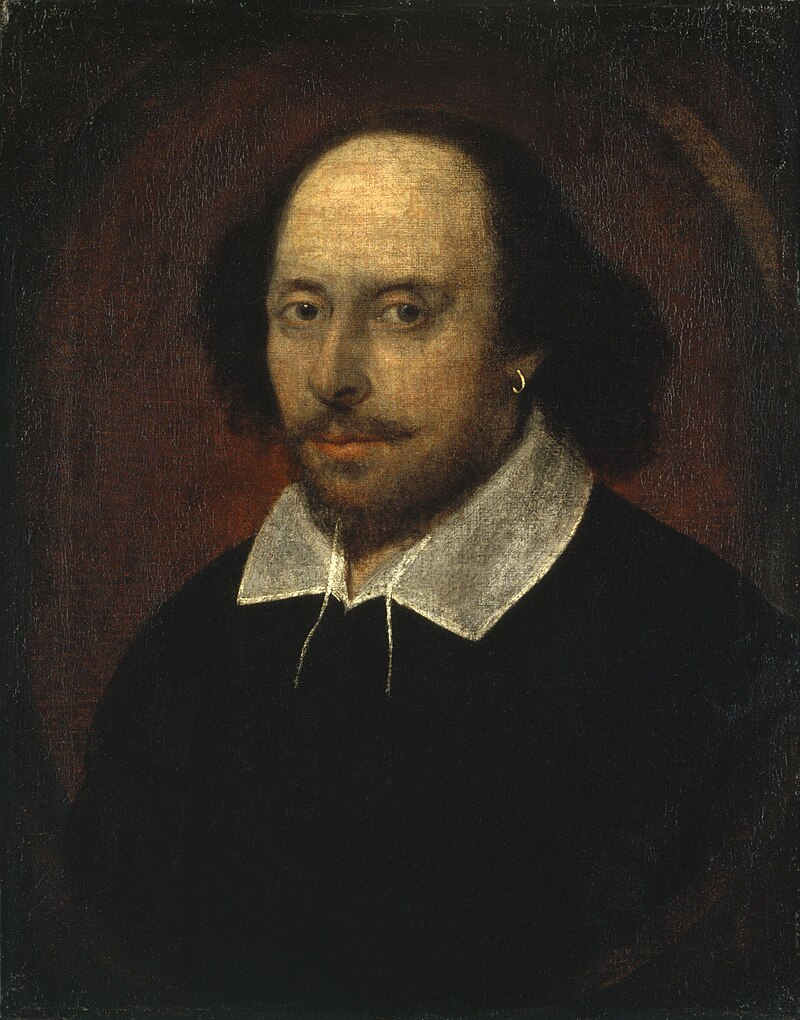
\includegraphics[height=4cm,alt={Portrait of William Shakespear}]{shake.jpg}
\includegraphics[height=4cm,artifact]{crinklepaper}\makebox[0pt][r]{Some text }


% If the document contains data tables, the author has to identify the header
% rows of the tables so that they can be tagged as <TH> cells. By default all
% cells are considered data cells. This can be done generally (in the preamble)
% or on a table by table basis before the table,
% as shown in the following example.

\tagpdfsetup{table/header-rows={1,2}}
\begin{tabular}{lr}
    % \multicolumn{2}{c}{Example}\\  % multicolumn raises compliance flags
    Name & Value \\
    This & 11 \\
    That & 2
\end{tabular}


% If a table should not be tagged as table, for example, because it is merely
% used to ensure that the content is properly aligned, it should be turned
% into a presentation table with the table/tagging=presentation key as shown
% below.

%\tagpdfsetup{table/tagging=presentation}
% \begin{tabular}{ccc}
%     \textbullet & \textbullet & \textbullet \\
%     --- & --- & ---
% \end{tabular}


% Most lists using standard LaTeX environments such as enumerate will be tagged
% automatically. The new list implementation also implement an optional
% key-value interface with similar features to the well known enumitem package,
% although with a different implementation.

\section{lists}

A list starting at 5

\begin{enumerate}[start=5]
\item Level A1
  \begin{enumerate}
  \item Level B1
  \item Level B2
  \end{enumerate}
\item Level A2
\end{enumerate}


Some text outside the list, then resume the list:

\begin{enumerate}[resume=true]
\item Level A1
  \begin{enumerate}
  \item Level B1
  \item Level B2
  \end{enumerate}
\item Level A2
\end{enumerate}


\section{Basic mathematical expressions}

If $x$ is real, then $x^{2} \geq 0$.

A matrix equation.
\[
\begin{pmatrix}0&1\\1&0\end{pmatrix}
\begin{pmatrix}a&b\\c&d\end{pmatrix}
=
\begin{pmatrix}c&d\\a&b\end{pmatrix}
\]


\end{document}

